\documentclass{article}

\PassOptionsToPackage{numbers,sort&compress,square}{natbib}
\usepackage[preprint]{neurips_2025}

\usepackage{natbib} % only if neurips_2025 did not already load it
\setcitestyle{numbers,square,comma}

\usepackage[utf8]{inputenc}
\usepackage[T1]{fontenc}

\usepackage{amsmath, amssymb, amsfonts, amsthm}
\usepackage{algorithm}
\usepackage{algpseudocode}

\usepackage{booktabs}
\usepackage{graphicx}
\usepackage{subcaption}
\usepackage{float}
\usepackage{xcolor}
\usepackage{microtype}
\usepackage{url}
\usepackage{hyperref}



% Only keep TikZ if you use the pipeline diagram.
\usepackage{tikz}
\usetikzlibrary{positioning, shapes.geometric, arrows.meta, fit, backgrounds}

\graphicspath{{figures/}}

\newtheorem{definition}{Definition}
\newtheorem{assumption}{Assumption}
\newtheorem{proposition}{Proposition}
\newtheorem{theorem}{Theorem}
\newtheorem{remark}{Remark}

\title{
Two-Level Contextual Bandits for Nurse Rostering:\\
A Construct-and-Repair Framework and Its Regime of Applicability
}

\author{
Ria Sonalker \quad Achuthan Rathinam \quad Jihyeon Yun \\
Computing and Data Science, Boston University \\
\texttt{\{rsonalk, achuthan, jihyeon\}@bu.edu}
}

\begin{document}

\maketitle

\begin{abstract}
We formulate the Second International Nurse Rostering Competition
(INRC-II) problem as a two-level contextual bandit problem: a bandit
policy selects among four construction heuristics to build a multi-week
schedule one week at a time, and a second bandit selects among $18$ repair
strategies to iteratively reduce constraint violations. Our pipeline
substantially outperforms a random-greedy baseline during construction
and further improves heuristically initialized schedules during repair.
Across the bandit algorithms we evaluated (LinUCB, UCB1, Thompson sampling,
$\varepsilon$-greedy, and uniform selection), \textbf{UCB1}
achieved the strongest week-level results. However, when applied to
near-optimal schedules from a branch-and-price solver, the repair stage
often degrades solution quality. This suggests that repair values are
strongly state-dependent: the best local edit depends on the current
schedule and on downstream edits it enables, a structure captured by a
Markov decision process but discarded by a bandit formulation. We
characterize this regime of applicability and motivate a full sequential
decision formulation as future work.
\end{abstract}

% ============================================================
\section{Introduction}
% ============================================================

Nurse rostering is a canonical NP-hard combinatorial optimization problem.
It requires assigning nurses to shifts across multiple weeks under hard
staffing rules and soft objectives over fairness, workload, and
preferences. Two families of methods dominate. Exact solvers such as
integer programming and branch-and-price produce high-quality schedules
at substantial computational cost. Fast constructive heuristics produce
schedules quickly but commit to a single fixed strategy regardless of
instance structure. Neither approach adapts to the fact that different
weeks in the same instance have different bottlenecks. One week may be
coverage-limited, another fatigue-limited, and another weekend-limited. A
heuristic chosen up front cannot exploit this variation.

This paper asks whether a learned policy can. We frame the problem as a
two-level contextual bandit, with one bandit at each stage of the
pipeline. A week-level bandit selects among construction heuristics to
build the schedule one week at a time, and a repair-level bandit selects
among local repair operators to iteratively reduce violations. At each
step, the active bandit observes a short feature vector summarizing the
current schedule, such as coverage gaps, workload distribution, and the
number of remaining violations, and selects which arm to apply next.

We chose contextual bandits over full reinforcement learning for practical
reasons. They train in minutes rather than hours, use a simple linear
model that is easy to debug, and come with well-understood theoretical
guarantees. The open question is whether this simplicity is enough for a
problem where each decision affects which future decisions are available.
That is the tradeoff this paper investigates.

% ============================================================
\section{Background and Related Work}
% ============================================================

\subsection{Nurse Rostering}

Nurse rostering is the problem of assigning a set of nurses to shifts over
a planning horizon while respecting regulatory, contractual, and operational
constraints. It is a well-studied member of the broader personnel
scheduling family and is NP-hard in its general form. Two foundational
surveys map the landscape of problem formulations and solution techniques.
\citet{cheang2003bibliographic} provide a bibliographic survey of nurse
rostering formulations, and \citet{burke2004state} survey the state of the
art of solution methods.

Approaches fall broadly into three groups. \emph{Exact methods} such as
integer linear programming and constraint programming encode the full
instance and can produce provably optimal schedules, but scale poorly with
instance size. \emph{Metaheuristics} such as tabu search, simulated
annealing, and variable neighborhood search navigate the combinatorial
space using neighborhood moves and acceptance criteria, and have been
competitive in international benchmarks. \emph{Hybrid methods} combine
mathematical programming with heuristic search. For example,
\citet{legrain2020rotation} introduce a rotation-based branch-and-price
formulation that produces high-quality reference solutions, and extend it
to an online stochastic variant in \citet{legrain2019online}. In our
experiments we use solutions from this branch-and-price line of work as a
near-optimal reference point.

\subsection{The INRC-II Benchmark}

The Second International Nurse Rostering Competition (INRC-II)
benchmark~\citep{ceschia2019inrc2} introduced a multi-stage (week-by-week)
formulation with a history component that propagates nurse state across
weeks. An instance specifies a scenario (nurse roster, skills, contracts),
a history (prior assignments at the start of the horizon), and a demand
file per week. Hard constraints enforce shift-succession legality, minimum
staffing, employee availability, and requested days off. Soft constraints
include optimal coverage, consecutive-work and rest patterns, complete
weekends, and preference satisfaction, each with a published weight. The
evaluation metric is the weighted sum of soft-constraint violations,
computed by an organizer-provided validator.

\subsection{Contextual Multi-Armed Bandits}

The multi-armed bandit framework models sequential decision-making under
uncertainty with bandit feedback. The contextual variant
\citep{lattimore2020bandit} provides the learner with a feature vector at
each round and asks it to select an arm based on that context. Two
algorithm families are standard. Upper-confidence-bound methods, beginning
with UCB1~\citep{auer2002finitetime}, select the arm whose estimated reward
plus an exploration bonus is highest. LinUCB~\citep{li2010contextual,chu2011contextual}
specializes this idea to linear reward models by maintaining a per-arm
ridge regression and choosing arms via an upper confidence ellipsoid.
Posterior-sampling methods follow Thompson's original proposal
\citep{thompson1933likelihood}; modern analyses for contextual linear
payoffs appear in \citet{agrawal2013thompson}. Adversarial settings admit
exponential-weights algorithms such as EXP3~\citep{auer2002nonstochastic}.
These methods typically assume rewards are independent draws from a fixed
(possibly context-dependent) distribution.

\subsection{Bandits for Algorithm and Operator Selection}

Our application is related to \emph{adaptive operator selection} and
\emph{algorithm selection}, which dynamically choose among heuristics or
neighborhood operators during search. \citet{fialho2010analysis} apply
multi-armed bandit algorithms to operator selection in evolutionary
algorithms, treating each operator as an arm and the quality gain it
produces as the reward. Hyper-heuristics~\citep{burke2013hyper} take a
complementary view and frame the problem as search over heuristics rather
than solutions. These approaches motivate bandits as a tool for selecting
among heuristics, but rely on the assumption that operator value can be
captured as a function of observable state. Our results suggest this
assumption is only partially valid for nurse rostering. Contextual bandits
learn useful marginal preferences over operators, but can miss the
state-dependent, sequential structure of repair actions.

\subsection{Positioning}

To our knowledge, contextual bandits have not been applied end-to-end to
INRC-II as both a construction and a repair mechanism. We introduce such a
two-level pipeline, compare contextual and non-contextual bandit
algorithms at both levels, and use branch-and-price reference solutions
\citep{legrain2020rotation} to characterize when the bandit formulation is
effective and when it is not.

% ============================================================
\section{Problem Setup}
% ============================================================

\subsection{INRC-II Instance and Schedule}

An INRC-II instance specifies (i) a set of nurses with contractual rules,
(ii) a planning horizon of $W$ weeks (so $|\mathcal{D}| = 7W$ days),
(iii) shift types, skills, and per-day coverage requirements, and
(iv) an initial history describing each nurse's carry-over state from the
previous horizon. The goal is to construct a feasible schedule that
minimizes a weighted sum of soft-constraint violations.

\paragraph{Sets.}
Let $\mathcal{N}$ be the set of nurses, $\mathcal{D}=\{1,\ldots,7W\}$ the
set of days, $\mathcal{F}$ the set of shift types, and $\mathcal{Q}$ the
set of skills. Each nurse $n\in\mathcal{N}$ has a skill set
$\mathcal{Q}_n \subseteq \mathcal{Q}$. For each day $d$, shift $f$, and
skill $q$, the instance provides a minimum required coverage
$\mu_{d,f,q}$ and an (optional) target/optimal coverage
$\nu_{d,f,q} \ge \mu_{d,f,q}$.

\paragraph{Schedule.}
A schedule is a mapping
\[
\sigma : \mathcal{N}\times\mathcal{D} \to \mathcal{F}\cup\{\varnothing\},
\]
where $\sigma(n,d)=\varnothing$ denotes that nurse $n$ is off on day $d$.
A schedule induces coverage counts
\[
c_{d,f,q}(\sigma)
= \bigl|\{\, n\in\mathcal{N} : \sigma(n,d)=f \text{ and } q\in\mathcal{Q}_n \,\}\bigr|.
\]
Hard feasibility requires (at minimum) (i) at most one shift per nurse per
day and (ii) minimum coverage $c_{d,f,q}(\sigma)\ge \mu_{d,f,q}$ for all
$(d,f,q)$, along with additional structural restrictions such as forbidden
shift successions. Our construction and repair operators are designed to
preserve these hard constraints.

\paragraph{History (carry-over state).}
Let $h_t$ denote the history entering week $t\in\{1,\ldots,W\}$,
summarizing each nurse's carry-over state needed to evaluate constraints
across week boundaries (e.g., last worked shift, current consecutive-work
and consecutive-rest streaks, cumulative assignments, and cumulative
worked weekends). The dataset provides $h_1$; for $t>1$, $h_t$ is updated
deterministically from $(h_{t-1},\sigma)$.

\subsection{Objective}

INRC-II scores a schedule by a weighted sum over seven soft constraints:
optimal coverage (S1), consecutive-work patterns (S2), consecutive days off
(S3), preferences (S4), complete weekends (S5), total assignments relative
to contract bounds (S6), and total worked weekends (S7). Let
$v_i(\sigma,h_1)$ denote the number of violations of soft constraint $i$
under schedule $\sigma$ and initial history $h_1$, and let $w_i$ be its
published weight. The total penalty is
\[
\mathcal{P}(\sigma,h_1) \;=\; \sum_{i=1}^{7} w_i\, v_i(\sigma,h_1).
\]
We use the official INRC-II weights throughout~\citep{ceschia2019inrc2}.
Our goal is to construct a feasible schedule $\sigma$ that minimizes
$\mathcal{P}(\sigma,h_1)$.

\subsection{Bandit Formulation}

We decompose schedule generation into two sequential decision stages, each
modeled as a contextual bandit.

\paragraph{Week-level bandit.}
For each week $t\in\{1,\ldots,W\}$, the learner observes a context vector
$x^{(w)}_t \in \mathbb{R}^{d_w}$ summarizing the current instance state
(e.g., demand and carry-over history), selects an arm
$a^{(w)}_t \in \{1,\ldots,K_w\}$ corresponding to a construction heuristic,
and applies it to extend the partial schedule through week $t$. Let
$\sigma_{\le t}$ denote the partial schedule after constructing weeks
$1,\ldots,t$ (and $\sigma_{\le 0}$ the empty schedule). We define the
week-level reward as the (scaled) penalty reduction from adding week $t$:
\[
r^{(w)}_t
\;=\;
\frac{\mathcal{P}(\sigma_{\le t-1},h_1)-\mathcal{P}(\sigma_{\le t},h_1)}
{\rho_w},
\]
where $\rho_w>0$ is a reward scale factor. A positive reward indicates
that the chosen construction arm decreased the overall penalty relative
to the prior partial schedule.

\paragraph{Repair-level bandit.}
After construction, a repair loop runs for up to $T$ repair rounds. At
repair round $j\in\{1,\ldots,T\}$, the learner observes a context
$x^{(r)}_j \in \mathbb{R}^{d_r}$ summarizing the current schedule and its
residual violations, selects a repair arm
$a^{(r)}_j \in \{1,\ldots,K_r\}$ corresponding to a local repair operator,
and applies it to \emph{mutate} the schedule into $\sigma_j$ while
preserving hard feasibility (with $\sigma_0$ the post-construction
schedule). The repair reward is
\[
r^{(r)}_j
\;=\;
\frac{\mathcal{P}(\sigma_{j-1},h_1)-\mathcal{P}(\sigma_j,h_1)}{\rho_r},
\]
with scale factor $\rho_r>0$.

\paragraph{Feedback.}
In both stages the learner observes bandit feedback: only the reward of
the chosen arm, never counterfactual rewards for unchosen arms. The two
bandits are trained independently and evaluated both jointly (full
pipeline) and in isolation (single-stage ablations). The repair-level
bandit is trained on schedules produced by the greedy initializer used at
inference time, matching the deployment distribution. Schedules produced
by a branch-and-price solver are used only at evaluation as an
out-of-distribution probe.

% ============================================================
\section{Methods}
% ============================================================

\subsection{Pipeline Overview}

Figure~\ref{fig:pipeline} summarizes the end-to-end architecture. An
INRC-II instance is loaded and preprocessed into scenario, initial-history,
and per-week demand structures. A week-level bandit then constructs a
multi-week schedule one week at a time by selecting among four construction
heuristics. A repair-level bandit subsequently runs for $N$ rounds; at each
round it selects among $18$ local repair operators and mutates the shared
schedule in place while preserving hard feasibility. Both stages share the
same underlying LinUCB update (Sec.~\ref{sec:linucb}) but operate on
distinct arm sets, context vectors, and reward scales.

During training, the pipeline is executed repeatedly across instances from
the training split, and the bandit parameters $(A_a, b_a)$ accumulate
across instances. At inference time, the learned parameters are frozen and
the pipeline is executed once per instance without updates.

\subsection{LinUCB}
\label{sec:linucb}

We use the disjoint-model LinUCB of \citet{li2010contextual,chu2011contextual}.
Each arm $a \in \{1,\ldots,K\}$ maintains a ridge-regression model over the
context $\mathbf{x} \in \mathbb{R}^d$ via an arm-specific design matrix
$A_a \in \mathbb{R}^{d\times d}$ and response vector $b_a \in \mathbb{R}^d$,
initialized to $A_a = I_d$ and $b_a = \mathbf{0}$. At each round, the arm
parameters and upper-confidence-bound score are
\[
\hat{\theta}_a = A_a^{-1} b_a,
\qquad
\mathrm{UCB}_a(\mathbf{x}) =
\hat{\theta}_a^\top \mathbf{x} +
\alpha \sqrt{\mathbf{x}^\top A_a^{-1} \mathbf{x}},
\]
and the learner pulls $a^\star = \arg\max_a \mathrm{UCB}_a(\mathbf{x})$.
After observing the scaled reward $\tilde{r} = r/\rho$, the update is
\[
A_{a^\star} \leftarrow A_{a^\star} + \mathbf{x}\mathbf{x}^\top,
\qquad
b_{a^\star} \leftarrow b_{a^\star} + \tilde{r}\,\mathbf{x}.
\]
The exploration coefficient $\alpha$ and reward scale $\rho$ are
hyperparameters (values in Sec.~\ref{sec:training}).

\subsection{Week-Level Bandit}

\paragraph{Arms.}
The week-level bandit selects among four construction heuristics
($K_w = 4$). Each arm iterates over nurses in an arm-specific priority
order and greedily fills the week's coverage requirements subject to hard
feasibility; the arms differ only in their nurse-priority key. The full
list appears in Appendix~\ref{app:week-arms}.

\paragraph{Context.}
At the start of each week the learner observes
$\mathbf{x}^{(w)}_t \in \mathbb{R}^{6}$ with components
\begin{align*}
x_1 &= \text{coverage\_slack}
  = \operatorname{clip}\!\left(\tfrac{\sum_{d,f,q}\mu_{d,f,q}}{|\mathcal{N}|\cdot 7},\, 0, 1\right), \\
x_2 &= \text{mean\_fatigue\_ratio}
  = \tfrac{1}{|\mathcal{N}|}\sum_n \tfrac{\texttt{consecWork}(n)}{C_n^{\max}}, \\
x_3 &= \text{weekend\_spread\_ratio}
  = \operatorname{clip}\!\left(\tfrac{\operatorname{std}_n(\texttt{weekendsWorked}(n))}{\max_n \texttt{weekendCap}(n)},\, 0, 1\right), \\
x_4 &= \text{request\_density}
  = \operatorname{clip}\!\left(\tfrac{|\text{shiftOffRequests}|}{|\mathcal{N}|},\, 0, 1\right), \\
x_5 &= \text{max\_assignment\_saturation}
  = \operatorname{clip}\!\left(\max_n \tfrac{\texttt{totalAssignments}(n)}{u_n},\, 0, 1\right), \\
x_6 &= \text{week\_position}
  = \tfrac{w}{W-1}.
\end{align*}
All features lie in $[0,1]$, so $\|\mathbf{x}^{(w)}_t\|_2 \le \sqrt{6}$.

\paragraph{Reward.}
After applying the selected arm to extend the partial schedule, the reward
\[
r^{(w)}_t
= \mathcal{P}(\sigma_{\le t-1}, h_1) - \mathcal{P}(\sigma_{\le t}, h_1)
\]
is scaled by $\rho_w$ and fed to the LinUCB update.

\subsection{Repair-Level Bandit}

\paragraph{Arms.}
The repair-level bandit selects among $18$ local-edit operators
($K_r = 18$). Each operator exposes a \texttt{find\_violations} routine
that returns the currently active violations it can address and an
\texttt{apply} routine that attempts a single feasibility-preserving edit.
Operators are grouped by the soft constraint they primarily target (four
for coverage, six for consecutive-work and consecutive-shift patterns,
three for consecutive days off, one for preferences, two for weekend
constraints, one for total assignments, and one catch-all random same-day
swap); the full list appears in Appendix~\ref{app:repair-arms}.

\paragraph{Context.}
The repair context $\mathbf{x}^{(r)}_j \in \mathbb{R}^{7}$ summarizes
which soft constraint dominates the current penalty and how far through
the repair loop the learner is. Let $P_j = \mathcal{P}(\sigma_j, h_1)$ and
let $P_j^{(S_i)}$ be the contribution from soft constraint $S_i$. Define
\[
x'_i = \tfrac{P_j^{(S_i)}}{\max(P_j, 1)}
       \ \text{for } i \in \{1, 2, 3, 4, 6\},
\quad
x'_5 = \tfrac{P_j^{(S_5)} + P_j^{(S_7)}}{\max(P_j, 1)},
\quad
x'_7 = \tfrac{j}{\max(N - 1, 1)}.
\]
The first six coordinates form a probability simplex when $P_j > 0$,
making the context instance-invariant: the bandit conditions on
\emph{which} constraint dominates, not on the absolute penalty magnitude,
which varies by an order of magnitude across \texttt{n030w4} and
\texttt{n120w4} instances.

\paragraph{Reward.}
The repair reward is the one-step penalty reduction
\[
r^{(r)}_j
= \mathcal{P}(\sigma_{j-1}, h_1) - \mathcal{P}(\sigma_j, h_1),
\]
scaled by $\rho_r$. Note that $r^{(r)}_j$ can be negative when an action
increases the soft penalty.

\subsection{Training Protocol}
\label{sec:training}

\paragraph{Initializer.}
The repair-level bandit is trained on schedules produced by the greedy
initializer used at inference time, matching the deployment distribution.
Schedules produced by a branch-and-price solver are used only at
evaluation, as an out-of-distribution probe (Sec.~\ref{sec:experiments}).

\paragraph{Instance streaming.}
Both bandits are trained across multiple instances drawn from the training
split. For each instance, the week-level bandit receives $W$ pulls (one per
week) and the repair-level bandit receives up to $N$ pulls (one per repair
round). Each bandit's parameters $(A_a, b_a)$ are accumulated across
instances; arm identities are fixed so that $\hat{\theta}_a$ has a
consistent meaning throughout training.

\paragraph{Warm start.}
To prevent LinUCB from collapsing onto a single arm before its per-arm ridge
models have sufficient data, we use a brief round-robin warm-start phase:
the first $W_{\text{warm}}$ pulls at each level cycle through arms
uniformly, after which the LinUCB rule takes over.

\paragraph{Hyperparameters.}
Unless otherwise stated we use $\alpha = 1.0$, $\rho_w = 1000$,
$\rho_r = 50$, $W_{\text{warm}} \in \{8, 36\}$ for the week and repair
levels respectively, and $N = 500$ repair rounds per instance.

\subsection{Baselines}

At both levels we compare LinUCB against non-contextual bandit algorithms
sharing the same arm set and reward signal but ignoring the context:
\textsc{Uniform}, \textsc{UCB1}~\citep{auer2002finitetime},
\textsc{Thompson}~\citep{thompson1933likelihood,agrawal2013thompson}, and
$\varepsilon$-greedy. All baselines use the same scaled reward
$\tilde{r} = r/\rho$ as LinUCB. This isolates the contribution of the
contextual term rather than changing the learning signal.

\subsection{Theoretical Considerations}

Both LinUCB and UCB1 come with well-known regret bounds. LinUCB's regret
grows as $\widetilde{O}(d\sqrt{T})$
\citep{li2010contextual,chu2011contextual,abbasi2011improved} and UCB1's as
$O(\sqrt{KT \log T})$ \citep{auer2002finitetime}. These bounds, however,
rest on assumptions that our setting violates.

Both algorithms assume the reward of each arm is drawn independently from a
fixed distribution (optionally depending on the observed context). In our
repair-level problem this assumption fails. The reward of a repair action
at round $j$ depends on the entire history of actions
$a^{(r)}_1,\ldots,a^{(r)}_j$ through their effect on the schedule
$\sigma_j$. Two pulls of the same arm with the same context vector can
yield different rewards if the underlying schedules are in different
states.

As a result, the cited bounds do not directly apply. Even if they did, they
would only compare our performance against the best policy that ignores
schedule state, a class that is strictly weaker than the state-dependent
policies the problem admits. Our out-of-distribution repair experiment
(Sec.~\ref{sec:ood-repair}) provides a lower bound on this gap by
contrasting LinUCB repair against leaving a near-optimal schedule
untouched.

% ------------------------------------------------------------
% Pipeline figure
% ------------------------------------------------------------

\begin{figure}[t]
\centering
\resizebox{\textwidth}{!}{%
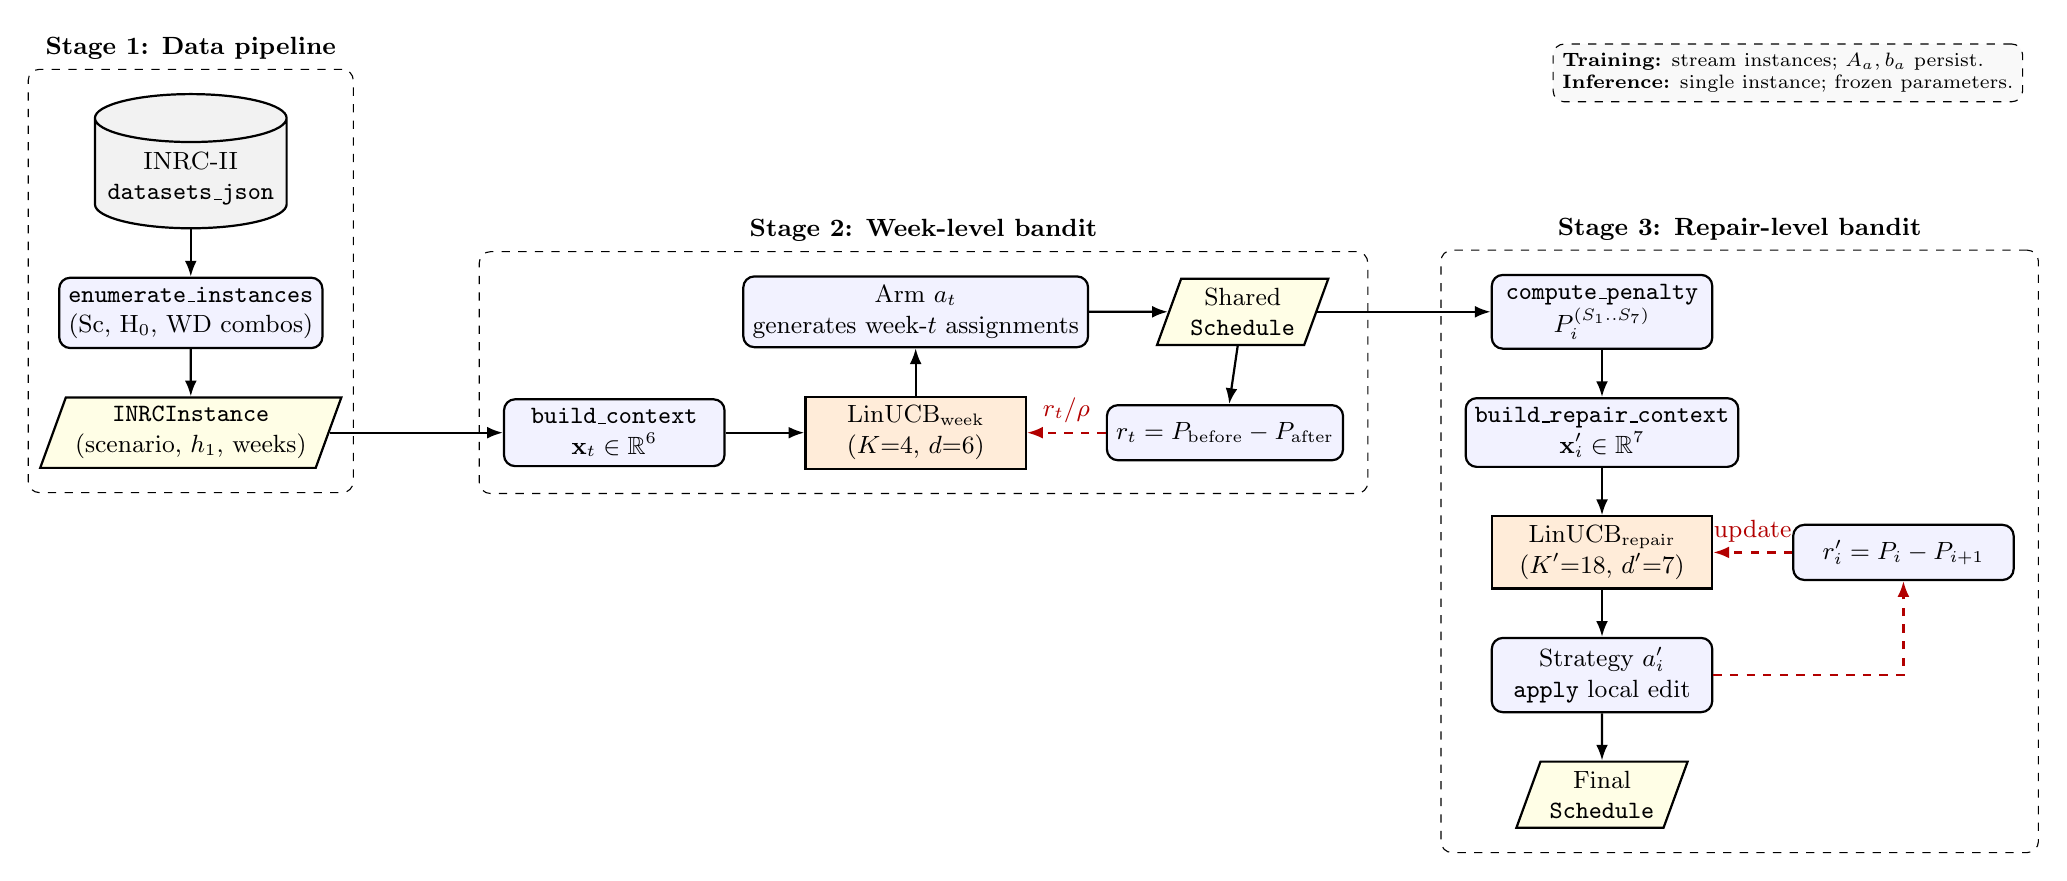
\begin{tikzpicture}[
  font=\small,
  node distance=6mm and 10mm,
  proc/.style   ={rectangle, rounded corners, draw, thick,
                  minimum width=28mm, minimum height=7mm,
                  align=center, fill=blue!5},
  data/.style   ={trapezium, trapezium left angle=70, trapezium right angle=110,
                  draw, thick, minimum width=20mm, align=center, fill=yellow!10},
  store/.style  ={cylinder, shape border rotate=90, aspect=0.25, draw, thick,
                  minimum height=12mm, minimum width=22mm,
                  align=center, text width=22mm, fill=gray!10},
  bandit/.style ={rectangle, draw, thick, minimum width=28mm, minimum height=9mm,
                  align=center, fill=orange!15},
  flow/.style   ={-{Latex[length=2mm]}, thick},
  reward/.style ={-{Latex[length=2mm]}, dashed, thick, red!70!black},
  stage/.style  ={draw, dashed, rounded corners, inner sep=3mm}
]

% ---------- Stage 1: vertical column ----------
\node[store] (ds) {INRC-II\\\texttt{datasets\_json}};
\node[proc, below=of ds]   (enum) {\texttt{enumerate\_instances}\\(Sc, H$_0$, WD combos)};
\node[data, below=of enum] (inst) {\texttt{INRCInstance}\\(scenario, $h_1$, weeks)};

% ---------- Stage 2 ----------
\node[proc, right=22mm of inst] (ctx1) {\texttt{build\_context}\\$\mathbf{x}_t \in \mathbb{R}^{6}$};
\node[bandit, right=of ctx1]    (lin1) {LinUCB$_{\text{week}}$\\$(K{=}4,\,d{=}6)$};
\node[proc,   above=of lin1]    (arm1) {Arm $a_t$\\generates week-$t$ assignments};
\node[data,   right=of arm1]    (sch1) {Shared\\\texttt{Schedule}};
\node[proc,   right=of lin1]    (pen1) {$r_t = P_{\text{before}} - P_{\text{after}}$};

% ---------- Stage 3 ----------
\node[proc, right=22mm of sch1] (pen2)  {\texttt{compute\_penalty}\\$P_i^{(S_1..S_7)}$};
\node[proc,   below=of pen2]    (ctx2)  {\texttt{build\_repair\_context}\\$\mathbf{x}'_i \in \mathbb{R}^{7}$};
\node[bandit, below=of ctx2]    (lin2)  {LinUCB$_{\text{repair}}$\\$(K'{=}18,\,d'{=}7)$};
\node[proc,   below=of lin2]    (apply) {Strategy $a'_i$\\\texttt{apply} local edit};
\node[data,   below=of apply]   (out)   {Final\\\texttt{Schedule}};
\node[proc,   right=of lin2]    (rew2)  {$r'_i = P_i - P_{i+1}$};

% ---------- Arrows ----------
\draw[flow] (ds)          -- (enum);
\draw[flow] (enum)        -- (inst);
\draw[flow] (inst.east)   -- (ctx1.west);

\draw[flow]   (ctx1)      -- (lin1);
\draw[flow]   (lin1)      -- (arm1);
\draw[flow]   (arm1)      -- (sch1);
\draw[flow]   (sch1)      -- (pen1);
\draw[reward] (pen1)      -- node[above]{$r_t/\rho$} (lin1);

\draw[flow]   (sch1.east) -- (pen2.west);

\draw[flow]   (pen2)      -- (ctx2);
\draw[flow]   (ctx2)      -- (lin2);
\draw[flow]   (lin2)      -- (apply);
\draw[flow]   (apply)     -- (out);
\draw[reward] (apply.east) -| (rew2.south);
\draw[reward] (rew2)      -- node[above]{update} (lin2);

% ---------- Stage boxes ----------
\begin{scope}[on background layer]
  \node[stage, fit=(ds)(enum)(inst),
        label=above:\textbf{Stage 1: Data pipeline}] {};
  \node[stage, fit=(ctx1)(lin1)(arm1)(pen1)(sch1),
        label=above:\textbf{Stage 2: Week-level bandit}] {};
  \node[stage, fit=(pen2)(ctx2)(lin2)(apply)(out)(rew2),
        label=above:\textbf{Stage 3: Repair-level bandit}] {};
\end{scope}

% ---------- Training annotation ----------
\node[draw, dashed, rounded corners, fill=gray!5, align=left,
      font=\scriptsize, anchor=north east]
      at ([xshift=-2mm,yshift=-2mm]current bounding box.north east)
      {\textbf{Training:} stream instances; $A_a,b_a$ persist.\\
       \textbf{Inference:} single instance; frozen parameters.};

\end{tikzpicture}}%
\caption{End-to-end pipeline. Stage~1 loads an INRC-II instance. Stage~2
runs the week-level LinUCB bandit: a 6-dimensional context $\mathbf{x}_t$
is built from the instance, the bandit picks one of four construction arms,
and the resulting weekly schedule is appended to the shared schedule.
Stage~3 runs the repair-level LinUCB bandit for $N$ rounds: a 7-dimensional
context $\mathbf{x}'_i$ is built from the current penalty breakdown, the
bandit picks one of 18 repair strategies, and the strategy mutates the
shared schedule in place. Dashed red arrows denote reward feedback fed to
the corresponding bandit's update.}
\label{fig:pipeline}
\end{figure}

% ============================================================
\section{Experiments}
\label{sec:experiments}
% ============================================================

\noindent\textbf{Evaluation protocol.}

We evaluate on the INRC-II dev split using the official total penalty
$\mathcal{P}$. For each configuration we report the mean final penalty
(after week-level construction and 500 repair rounds) and, when relevant,
the mean repair improvement $\Delta = P_{\text{after week}} - P_{\text{after repair}}$.
Unless stated otherwise we follow the training protocol in
Sec.~\ref{sec:training}. Across the held-out splits and seeds we evaluated,
the standard deviation of mean final penalty was small relative to the
between-configuration differences we report, so we present point estimates
without error bars throughout.

\subsection{End-to-end comparison of bandit algorithms } % (Exp.~02)
\label{sec:exp2}

\begin{figure}[t]
    \centering
    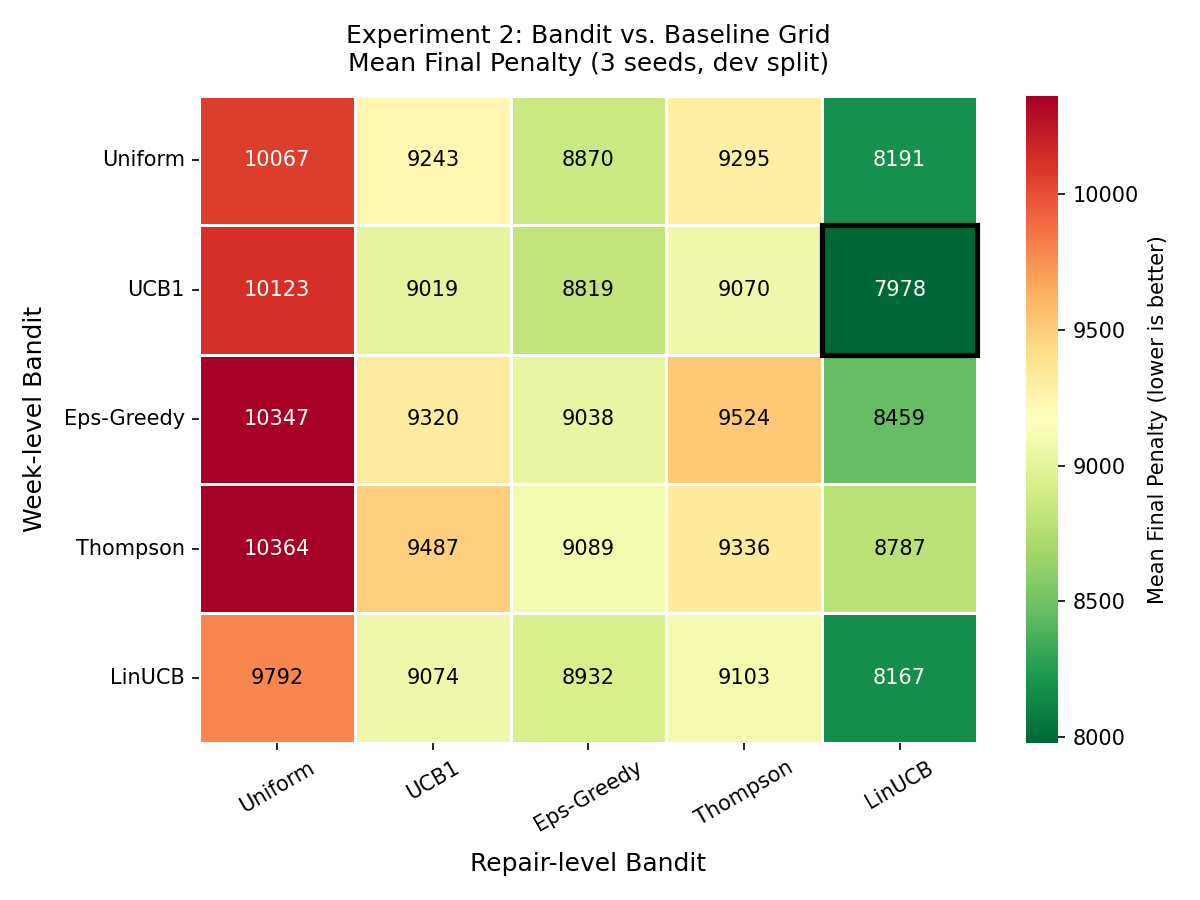
\includegraphics[width=0.60\textwidth]{experiment plots/experiment-02/exp2_heatmap.png}
    \caption{Mean final penalty (dev) for every week-level $\times$ repair-level
    bandit pair. Lower is better. The black border marks the best-performing
    combination.}
    \label{fig:exp2_heatmap}
\end{figure}

Figure~\ref{fig:exp2_heatmap} compares all $5\times 5$ combinations of the
week- and repair-level bandit algorithms described in Sec.~\ref{sec:linucb}
(Uniform, UCB1, $\varepsilon$-greedy, Thompson sampling, and LinUCB), using
the same arm sets ($K_w{=}4$ construction heuristics and $K_r{=}18$ repair
operators) and the same reward definition (penalty reduction).
Across week-level choices, LinUCB is consistently the strongest repair-level
method, indicating that conditioning repair decisions on schedule context is
valuable when the action space is large. In contrast, week-level performance
varies less across algorithms, consistent with the small number of weekly
decisions per instance. Overall, the best end-to-end performance is achieved
by the \textsc{UCB1} (week) $\times$ \textsc{LinUCB} (repair) pair, highlighted
in Fig.~\ref{fig:exp2_heatmap}.

\paragraph{Why does the best pair win?}
A plausible explanation is that the two stages have very different
decision regimes. At the week level there are only $K_w=4$ arms and only
$W$ pulls per instance, so non-contextual exploration (e.g., UCB1) can
identify a strong construction heuristic with little data, and the added
variance from fitting a contextual model may not pay off. In contrast, at
the repair level the action space is much larger ($K_r=18$) and the bandit
acts for many rounds (500), so conditioning on the current violation
profile can avoid wasting pulls on operators that are irrelevant in the
current schedule state. This interpretation is consistent with the
context-ablation results (Exp.~09) and with the observation that repair
behavior depends strongly on the starting schedule distribution
(Exp.~11).

\subsection{Is construction adaptivity needed? (Week-level cumulative reward)}
\label{sec:week-adaptivity}

\begin{figure}[t]
    \centering
    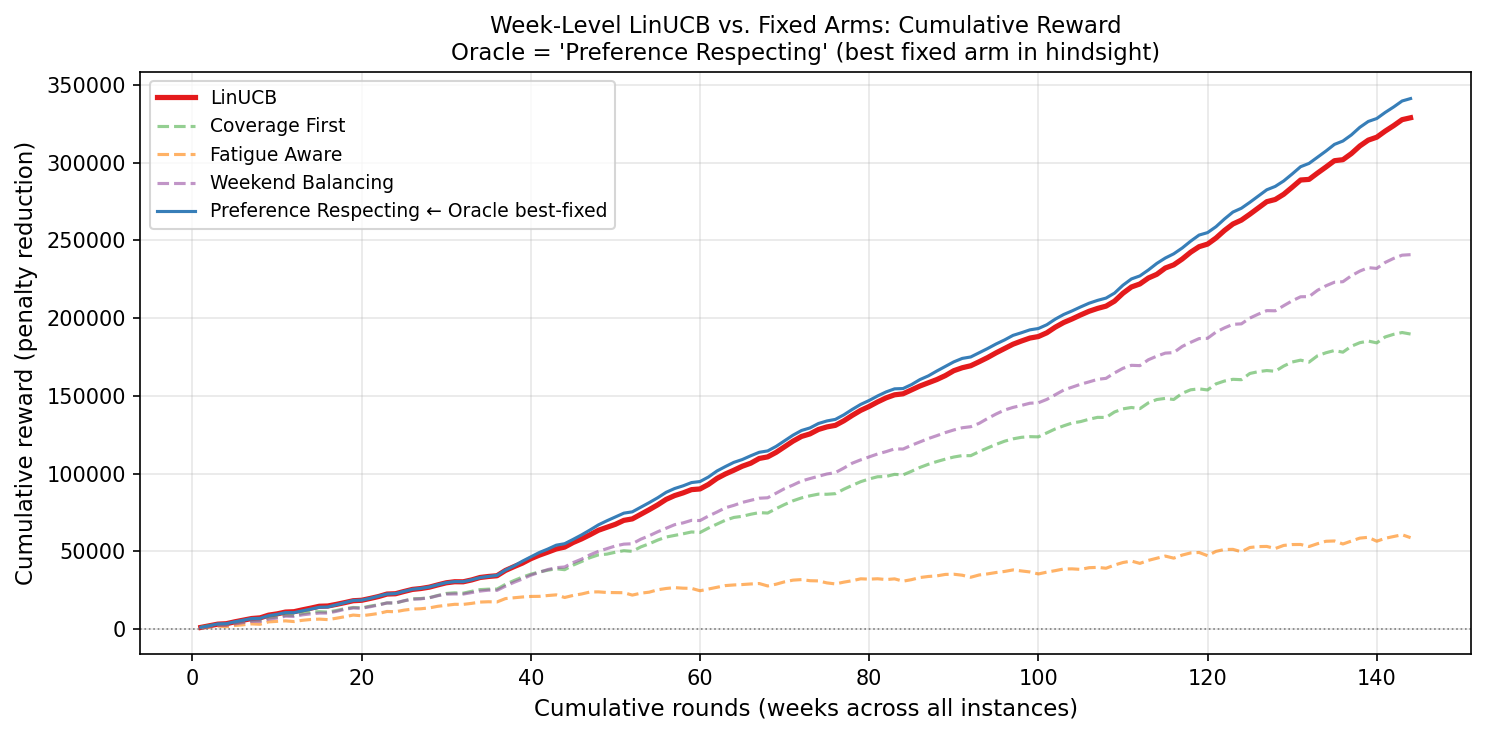
\includegraphics[width=0.70\textwidth]{experiment plots/exp: adaptive vs fixed cumilative/cumulative_reward.png}
    \caption{Week-level LinUCB versus fixed construction heuristics. Curves
    show cumulative reward (total penalty reduction) aggregated over all
    week decisions across the evaluated instances. The best fixed arm in
    hindsight is shown as an oracle baseline.}
    \label{fig:week_cum_reward}
\end{figure}

Because the week-level bandit makes only one decision per week (Sec.~3),
it receives relatively few pulls per instance. We therefore compare the
adaptive LinUCB construction policy against fixed-arm policies that use a
single construction heuristic for every week. Figure~\ref{fig:week_cum_reward}
plots cumulative reward (penalty reduction) over the sequence of week-level
decisions aggregated across instances. LinUCB tracks the oracle best-fixed
arm closely, suggesting that in this regime adaptivity provides limited
additional benefit beyond selecting a strong construction heuristic, and
helping explain why non-contextual week-level methods can be competitive
in the end-to-end comparison (Exp.~02).

\subsection{Context ablation (Exp.~09)}
\label{sec:context-ablation}

\begin{figure}[t]
    \centering
    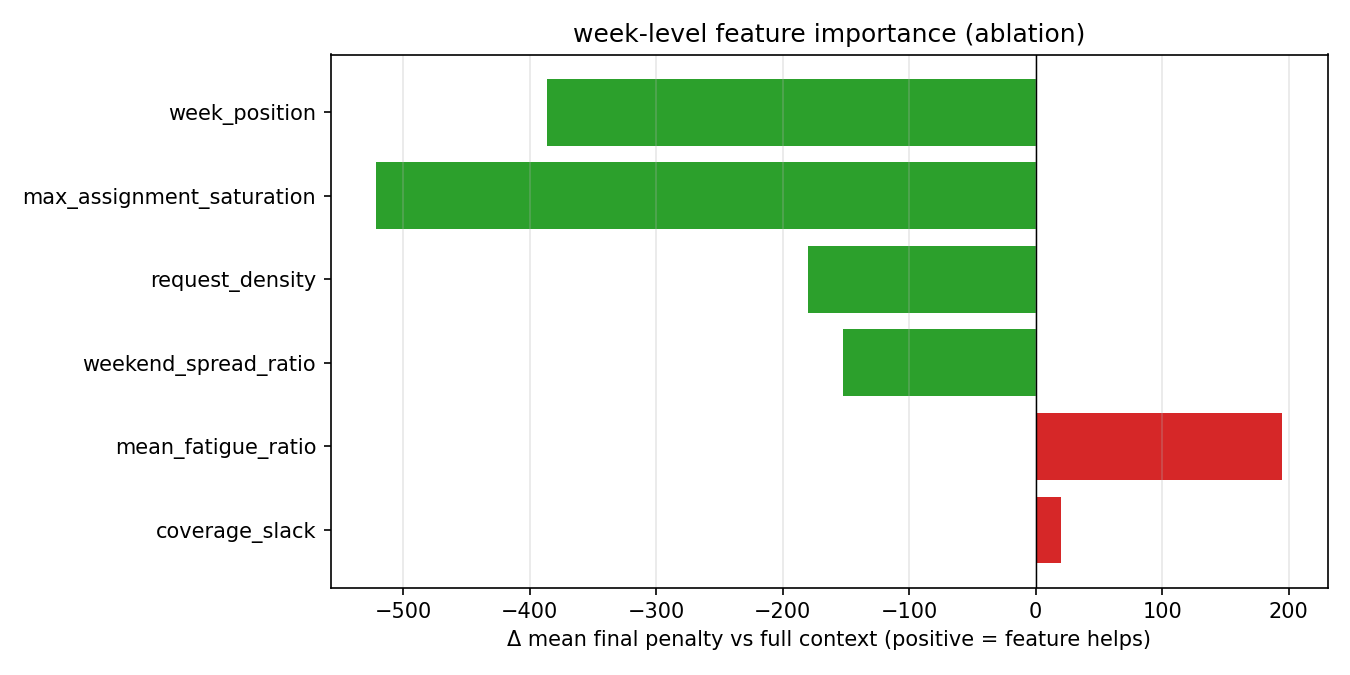
\includegraphics[width=0.48\textwidth]{experiment plots/experiment-09/ablation_week.png}
    \hfill
    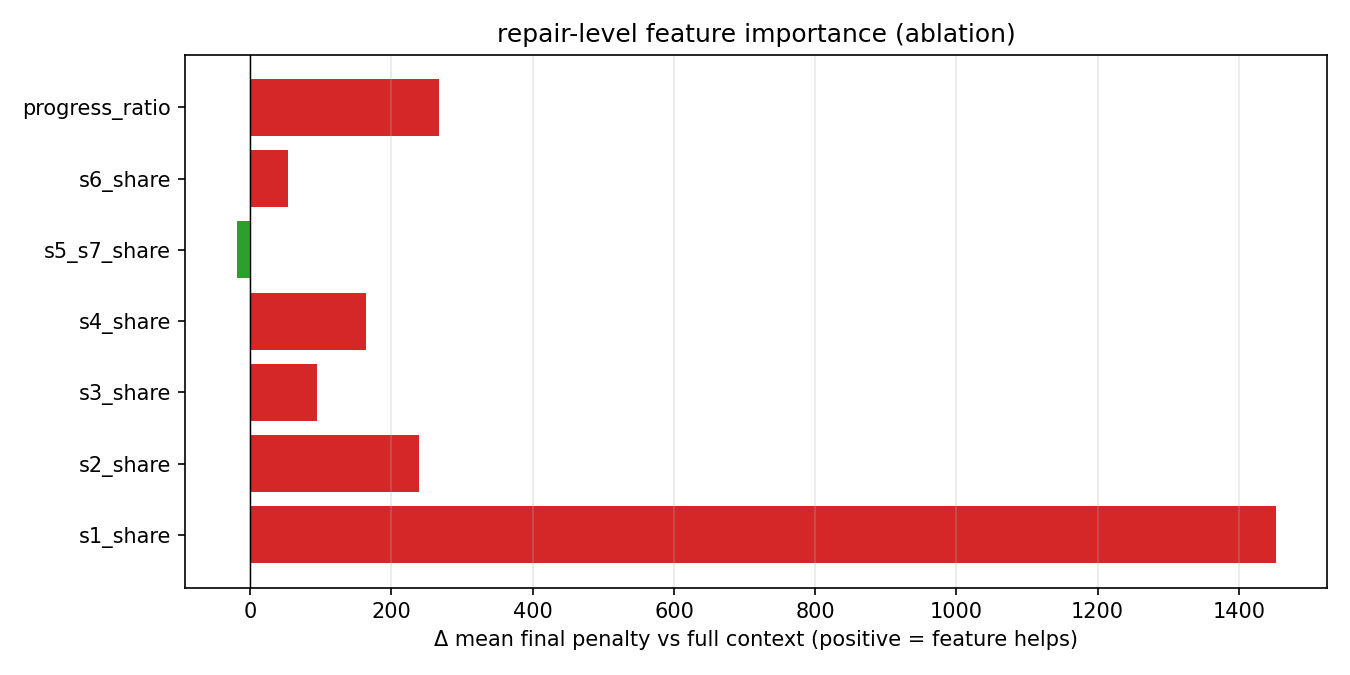
\includegraphics[width=0.48\textwidth]{experiment plots/experiment-09/ablation_repair.png}
    \caption{Context-feature ablation for the week-level bandit (left) and
    repair-level bandit (right). Each bar masks one feature while retraining
    LinUCB from scratch. Lower final penalty is better.}
    \label{fig:context-ablation}
\end{figure}

LinUCB’s advantage at the repair stage (Exp.~02) relies on the assumption
that the context vectors in Sec.~3 capture actionable information about the
current schedule. To test this, we perform a leave-one-feature-out ablation:
for each coordinate of the context vector, we retrain LinUCB with that
feature masked (set to zero) while keeping the training protocol fixed.
Figure~\ref{fig:context-ablation} shows that removing individual features
degrades performance, with a larger effect at the repair level than at the
week level. This supports the interpretation that contextual information is
most valuable when the decision space is large and the schedule state
changes substantially across rounds, as in the repair loop.

\paragraph{Outcome.}
Figure~\ref{fig:context-ablation} indicates that context is substantially more
useful at the repair level than at the week level. For construction, several
features have near-zero or negative contribution (i.e., masking them does not
hurt and can slightly improve mean final penalty), suggesting that the
week-level context may be noisy relative to the small number of decisions per
instance. In contrast, at repair the performance drop from masking
\texttt{s1\_share} (coverage-dominance) is by far the largest, with smaller but
nontrivial contributions from the other penalty-share coordinates and the
progress feature. This implies that the repair policy relies heavily on the
current violation profile to select among the 18 operators, consistent with
the end-to-end results in Exp.~02.

\subsection{Sensitivity and training protocol (Exps.~03--06)}
\label{sec:sensitivity}

We next stress-test the training protocol hyperparameters introduced in
Sec.~\ref{sec:training}. We retrain LinUCB from scratch while varying (i) the
exploration coefficient $\alpha$, (ii) reward scaling $\rho$, (iii) the number
of warm-start rounds, and (iv) the number of training instances used to
accumulate the per-arm ridge statistics, holding all other settings fixed.
Across these sweeps, week-level performance is comparatively stable, while
repair-level performance is more sensitive to hyperparameters, consistent with
the larger repair action space ($K_r=18$) and longer horizon (500 rounds).
Detailed sweep plots and values are reported in Appendix~\ref{app:sensitivity}
(Figs.~\ref{fig:app-alpha}--\ref{fig:app-data-scaling}).

\textbf{Exp.~03 (LinUCB exploration $\alpha$).} Sweeping $\alpha$ while holding the
rest of the protocol fixed yields smooth changes in held-out performance at both
levels, with no unstable settings; the repair stage shows a mild preference for
larger $\alpha$, consistent with the larger operator space ($K_r{=}18$) where
premature exploitation is costly.
\par\noindent\textbf{Exp.~04 (reward scaling $\rho$).} Varying the reward scale
$\rho$ (used to normalize penalty reductions before LinUCB updates) shows a
monotonic improvement with $\rho_w$ at the week level over the tested range, but
a non-monotonic response in $\rho_r$ at the repair level, indicating that repair
learning is more sensitive to reward normalization (which changes the balance
between the linear term $\hat{\theta}_a^\top x$ and the exploration bonus).
\par\noindent\textbf{Exp.~05 (warm-start length).} Introducing a short round-robin
warm start improves performance relative to zero warm start, suggesting that a
minimum amount of per-arm data prevents early collapse to a suboptimal arm;
beyond that point, gains diminish and the best warm-start length differs between
construction and repair.
\par\noindent\textbf{Exp.~06 (training-set scaling).} Increasing the number of
training instances generally improves week-level generalization, while repair
performance is less stable with train size, consistent with greater heterogeneity
in schedule states and operator effects across instances. (Note: in week-level
sweeps, $\Delta$ corresponds to cumulative penalty reduction from the empty-schedule
baseline within week construction; in repair-level sweeps, $\Delta$ is improvement
from the greedy-initialized schedule.)


\subsection{Regime of applicability: out-of-distribution repair starts (Exp.~11)}
\label{sec:ood-repair}

\begin{figure}[t]
    \centering
    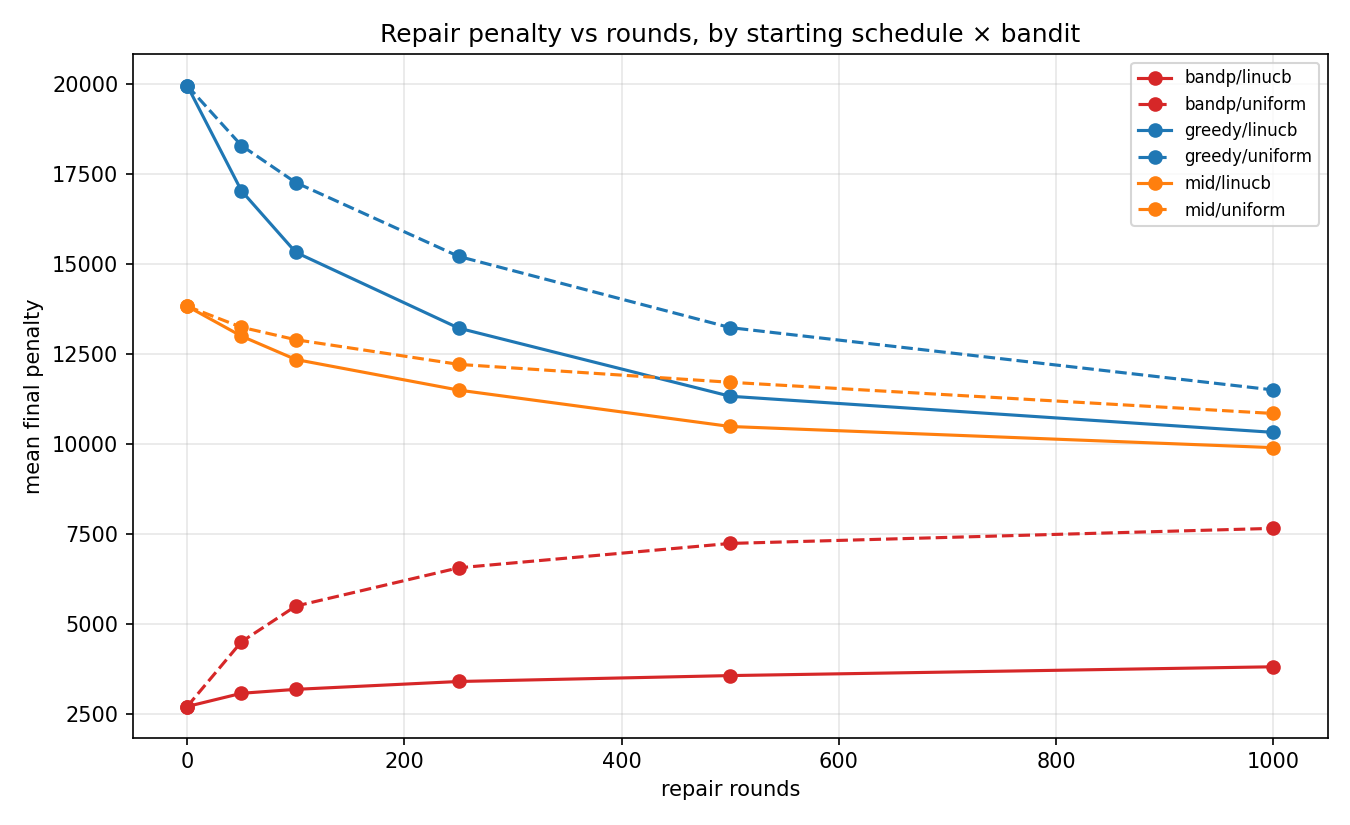
\includegraphics[width=0.62\textwidth]{experiment plots/experiment-11/ood_curves.png}
    \caption{Repair penalty versus repair rounds under different starting-schedule
    distributions. We compare LinUCB repair to uniform selection when starting from
    the greedy initializer (in-distribution), a ``mid'' start (greedy repaired for
    200 rounds by LinUCB), and bundled near-optimal solver schedules (bandp).}
    \label{fig:ood-curves}
\end{figure}

The repair bandit is trained on greedy-initialized schedules (Sec.~\ref{sec:training}),
so its learned values may not transfer to different starting states. As shown in
Fig.~\ref{fig:ood-curves}, LinUCB repair improves greedy and mid starts, but degrades
near-optimal solver starts as the number of repair rounds increases. This highlights
a regime where the value of a local edit is strongly state-dependent and where a
bandit abstraction that discards long-horizon effects can be insufficient.

% ============================================================
\section{Discussion and Future Work}
% ============================================================

The OOD result in Sec.~\ref{sec:ood-repair} is our central finding: the
contextual bandit formulation is effective when local edits monotonically
reduce a large pool of violations, but breaks down once the schedule is
near-optimal and the right action is often \emph{no action}. A bandit policy
cannot represent ``stop'' as a function of context alone, because the
penalty-share simplex looks similar in well-shaped schedules with very
different absolute quality. This is structural, not a matter of more data
or a better feature: it is the gap between bandit and Markov decision
process formulations.

Three directions follow naturally. First, recasting repair as an MDP with
the schedule as state and a stop action would close the gap our OOD
experiment quantifies. Second, a lightweight intermediate is to allow
online LinUCB updates during inference so the repair bandit can adapt to
each instance's starting distribution. Third, the week-level result in
Sec.~\ref{sec:week-adaptivity} suggests that contextual reasoning has the
most leverage when the action space is large and the horizon is long;
expanding the construction arm set would be a cheap way to test whether
the same regime appears at the week level.

\clearpage
\bibliographystyle{unsrtnat}
\bibliography{refs}


\clearpage

% ============================================================
\section*{Appendix}
% ============================================================
\addcontentsline{toc}{section}{Appendix}

\appendix

\section{Week-Level Arms}
\label{app:week-arms}

\begin{center}
\small
\begin{tabular}{cll}
\toprule
Arm & Strategy & Priority \\
\midrule
1 & \texttt{coverage\_first}        & Lowest-penalty nurse first; fills minimum coverage \\
2 & \texttt{fatigue\_aware}         & Rested nurses first; avoids long work streaks \\
3 & \texttt{weekend\_balancing}     & Equalizes weekends worked across nurses \\
4 & \texttt{preference\_respecting} & Honors shift-off requests where feasible \\
\bottomrule
\end{tabular}
\end{center}
\begin{center}
\small\textbf{Table A.1:} Week-level construction arms ($K_w = 4$).
\end{center}

\section{Repair-Level Operators}
\label{app:repair-arms}

\begin{center}
\small
\begin{tabular}{cll}
\toprule
Arm & Strategy & Target \\
\midrule
1  & \texttt{pull\_off\_day\_nurse}                 & S1 (coverage) \\
2  & \texttt{move\_same\_day\_surplus\_to\_deficit} & S1 \\
3  & \texttt{pull\_from\_adjacent\_day\_surplus}    & S1 \\
4  & \texttt{skill\_reassignment}                   & S1 \\
5  & \texttt{break\_long\_work\_streak\_mid}        & S2 (consecutive) \\
6  & \texttt{break\_long\_work\_streak\_start}      & S2 \\
7  & \texttt{break\_long\_work\_streak\_end}        & S2 \\
8  & \texttt{extend\_short\_work\_streak}           & S2 \\
9  & \texttt{break\_long\_same\_shift\_streak}      & S2 \\
10 & \texttt{extend\_short\_same\_shift\_streak}    & S2 \\
11 & \texttt{break\_long\_rest\_mid}                & S3 (days off) \\
12 & \texttt{break\_long\_rest\_boundary}           & S3 \\
13 & \texttt{extend\_short\_rest}                   & S3 \\
14 & \texttt{swap\_off\_unwanted\_shift}            & S4 (preferences) \\
15 & \texttt{reduce\_overloaded\_weekends}          & S5/S7 (weekends) \\
16 & \texttt{fix\_incomplete\_weekend}              & S5/S7 \\
17 & \texttt{rebalance\_overworked\_nurse}          & S6 (totals) \\
18 & \texttt{random\_feasible\_same\_day\_swap}     & any (catch-all) \\
\bottomrule
\end{tabular}
\end{center}
\begin{center}
\small\textbf{Table B.1:} Repair-level operators ($K_r = 18$).
\end{center}

\clearpage

\section{Sensitivity and training protocol details (Exps.~03--06)}
\label{app:sensitivity}

\begin{figure}[t]
    \centering
    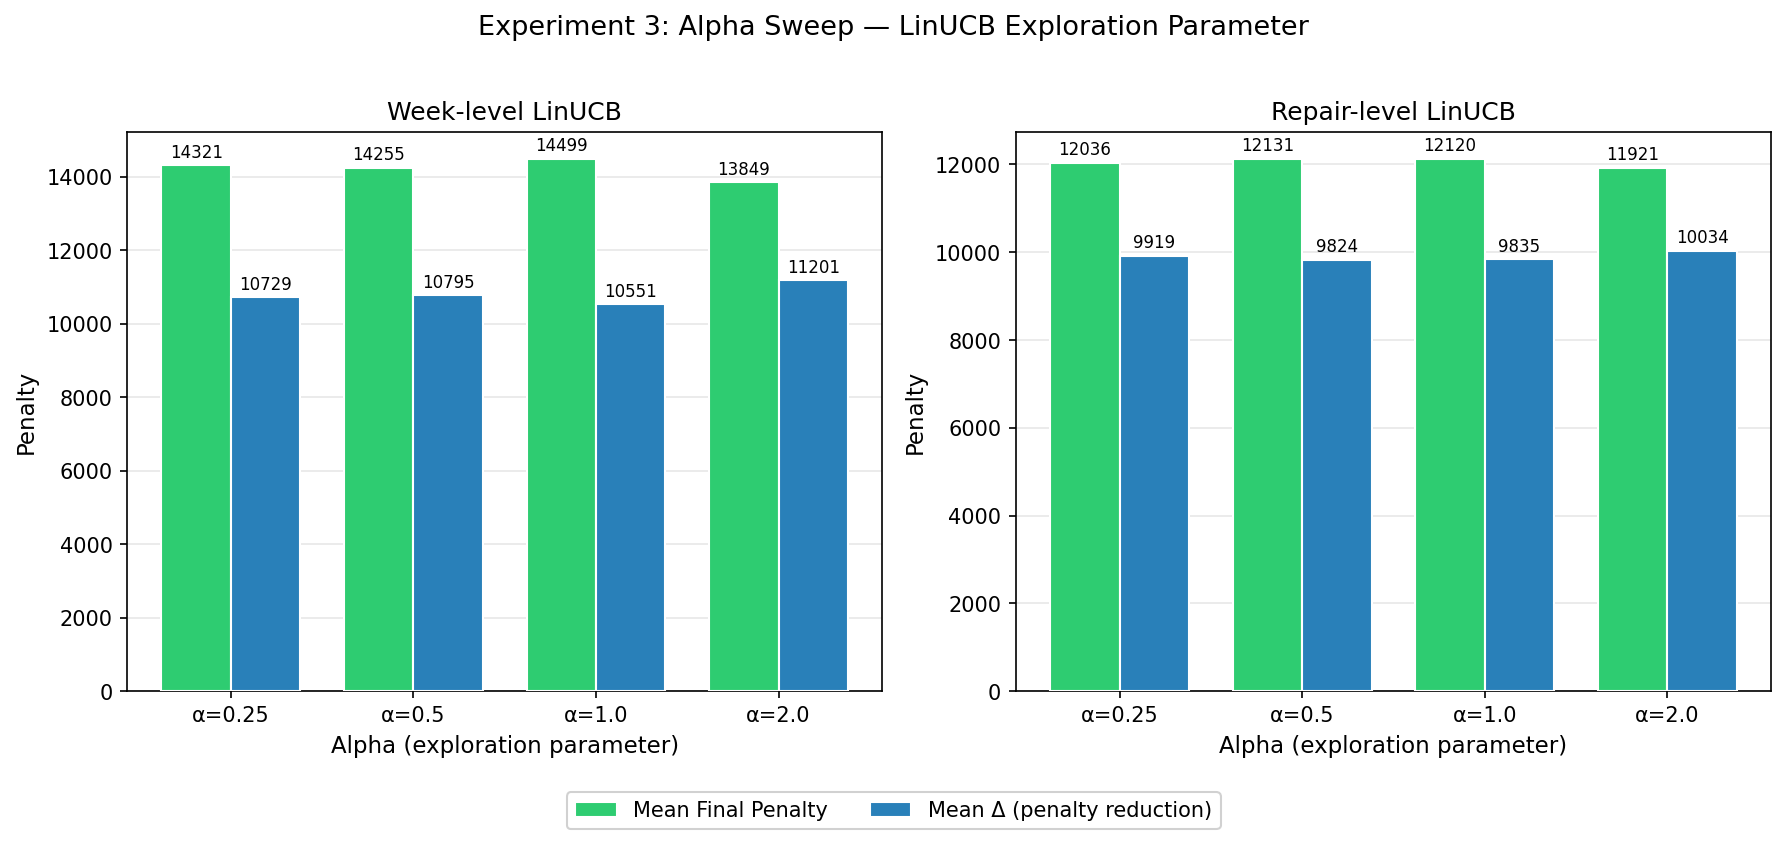
\includegraphics[width=0.65\textwidth]{experiment plots/experiment-03/exp3_alpha_sweep.png}
    \caption{Sensitivity to the LinUCB exploration coefficient $\alpha$ at the week
    level (left) and repair level (right).}
    \label{fig:app-alpha}
\end{figure}

\begin{figure}[t]
    \centering
    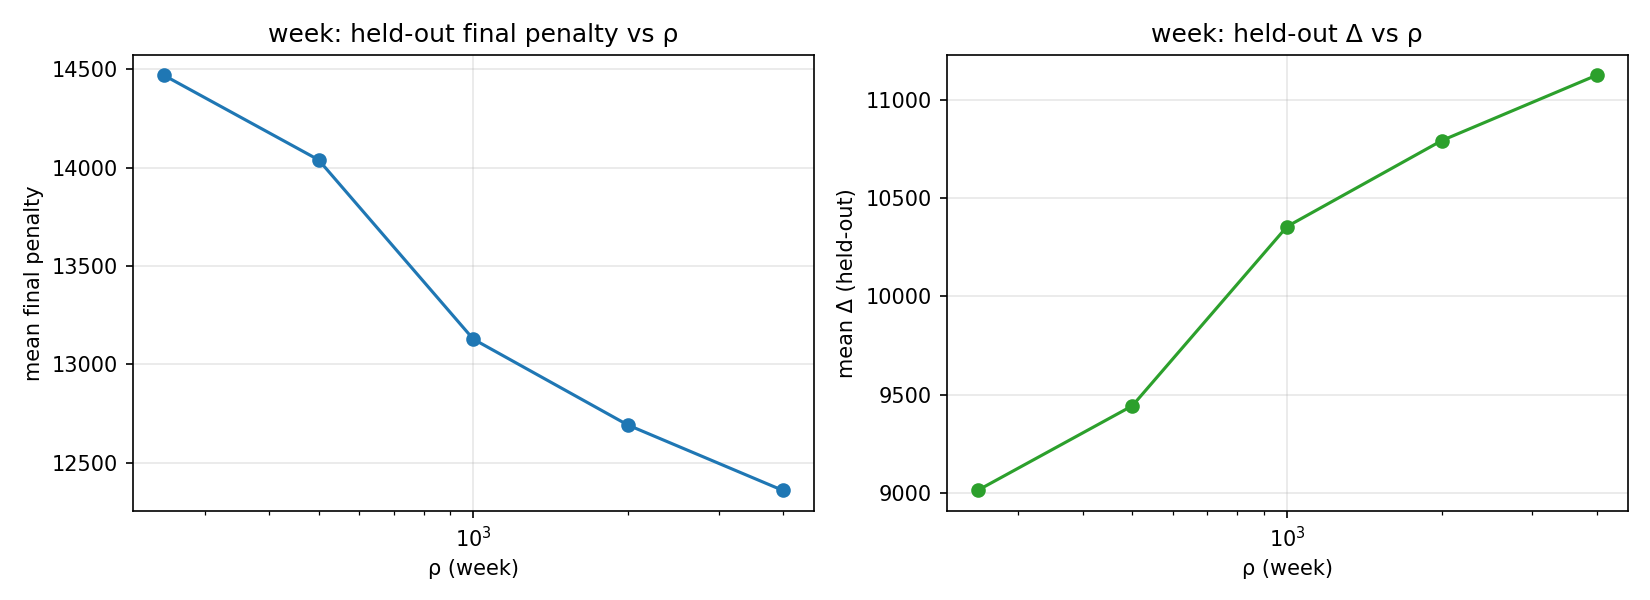
\includegraphics[width=0.48\textwidth]{experiment plots/experiment-04/reward_scale_week.png}
    \hfill
    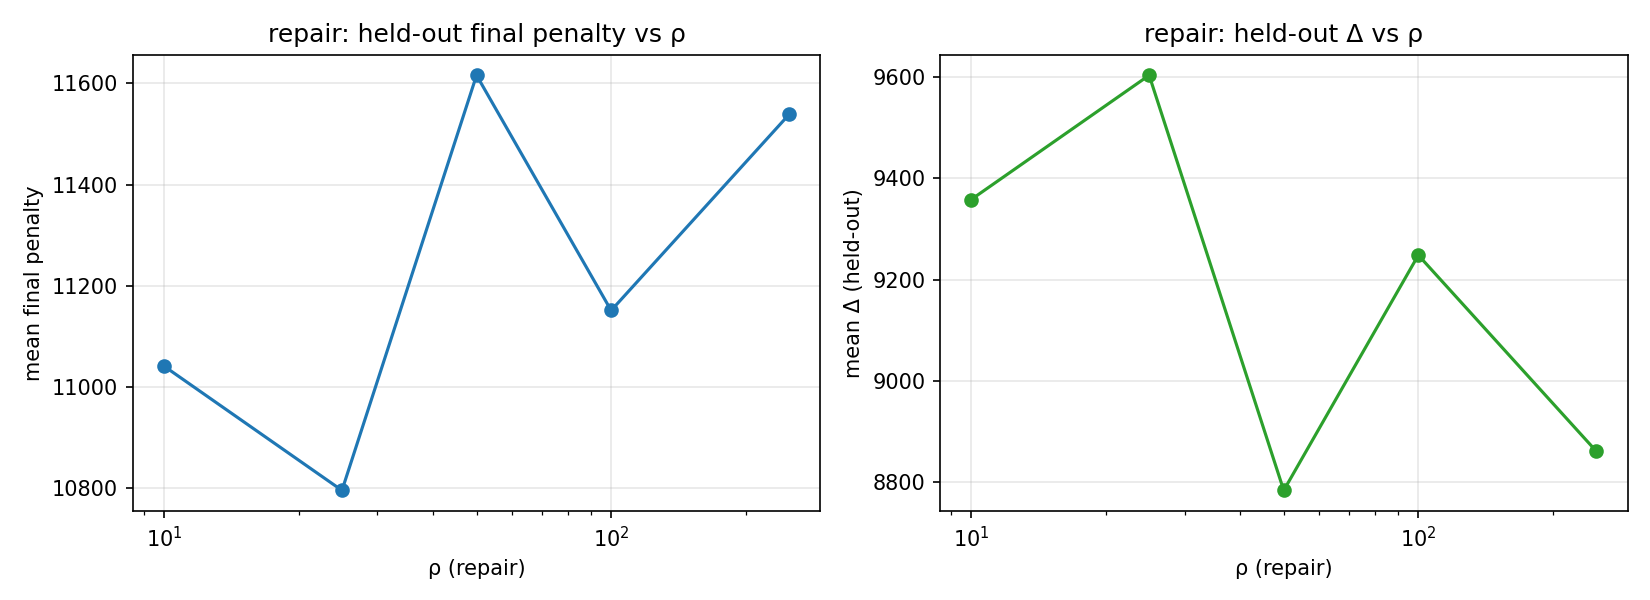
\includegraphics[width=0.48\textwidth]{experiment plots/experiment-04/reward_scale_repair.png}
    \caption{Reward-scale sensitivity: held-out dev mean final penalty and mean $\Delta$
    vs.\ reward scale $\rho$ at the week level (left) and repair level (right).}
    \label{fig:app-reward-scale}
\end{figure}


\begin{figure}[t]
    \centering
    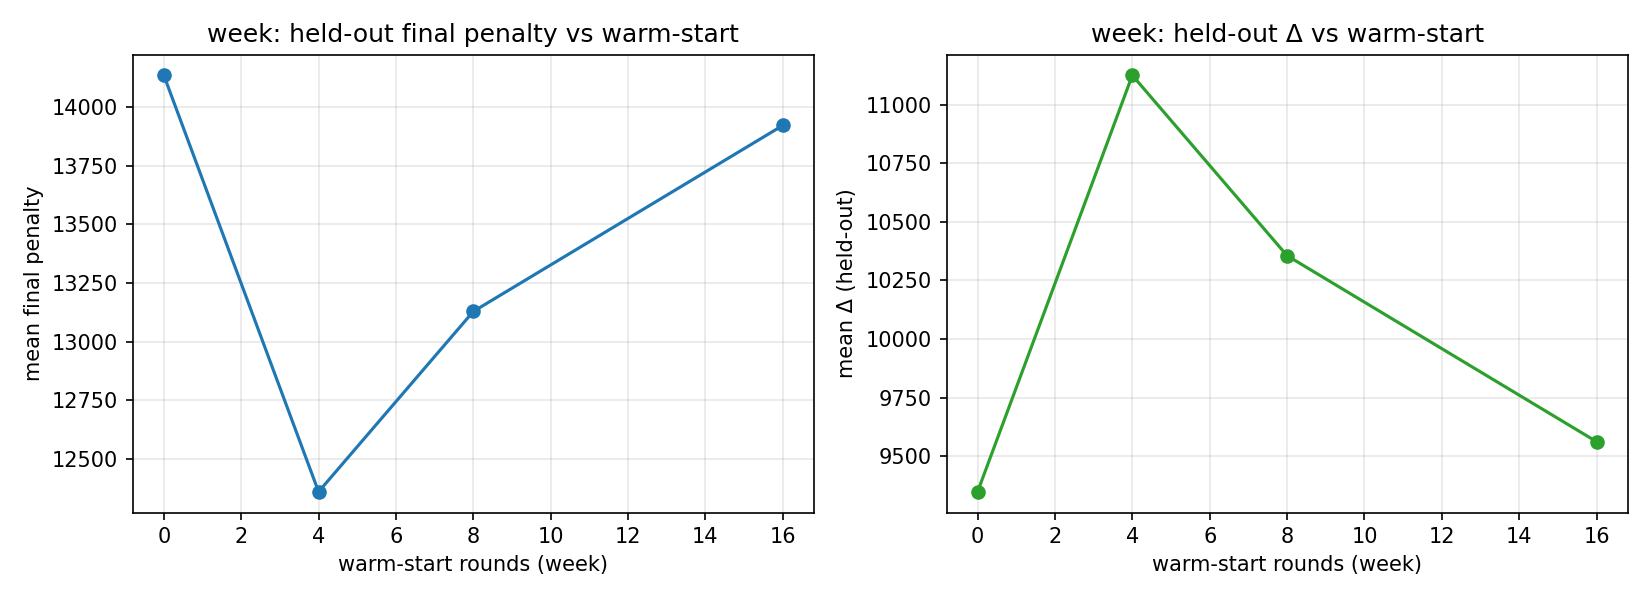
\includegraphics[width=0.48\textwidth]{experiment plots/experiment-05/warm_start_week.png}
    \hfill
    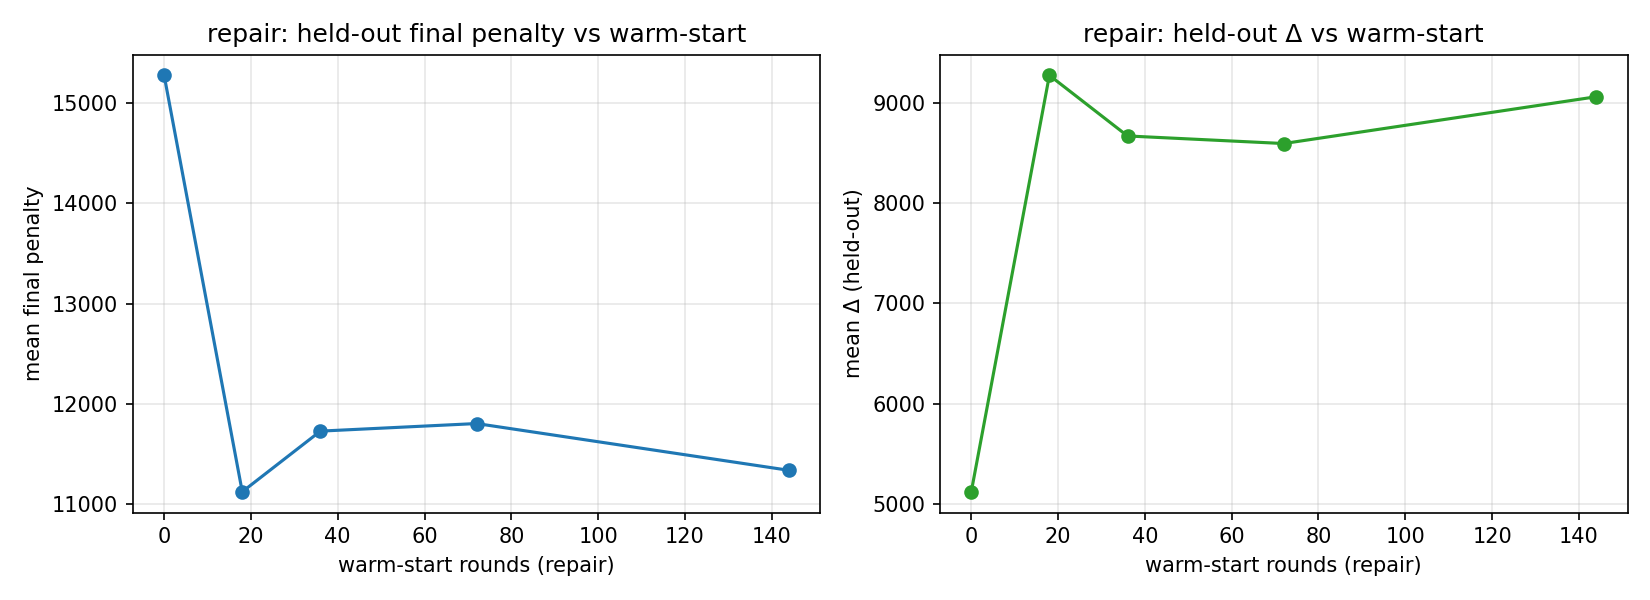
\includegraphics[width=0.48\textwidth]{experiment plots/experiment-05/warm_start_repair.png}
    \caption{Warm-start length: held-out dev mean final penalty and mean $\Delta$
    vs.\ warm-start rounds at the week level (left) and repair level (right).}
    \label{fig:app-warm-start}
\end{figure}

\begin{figure}[t]
    \centering
    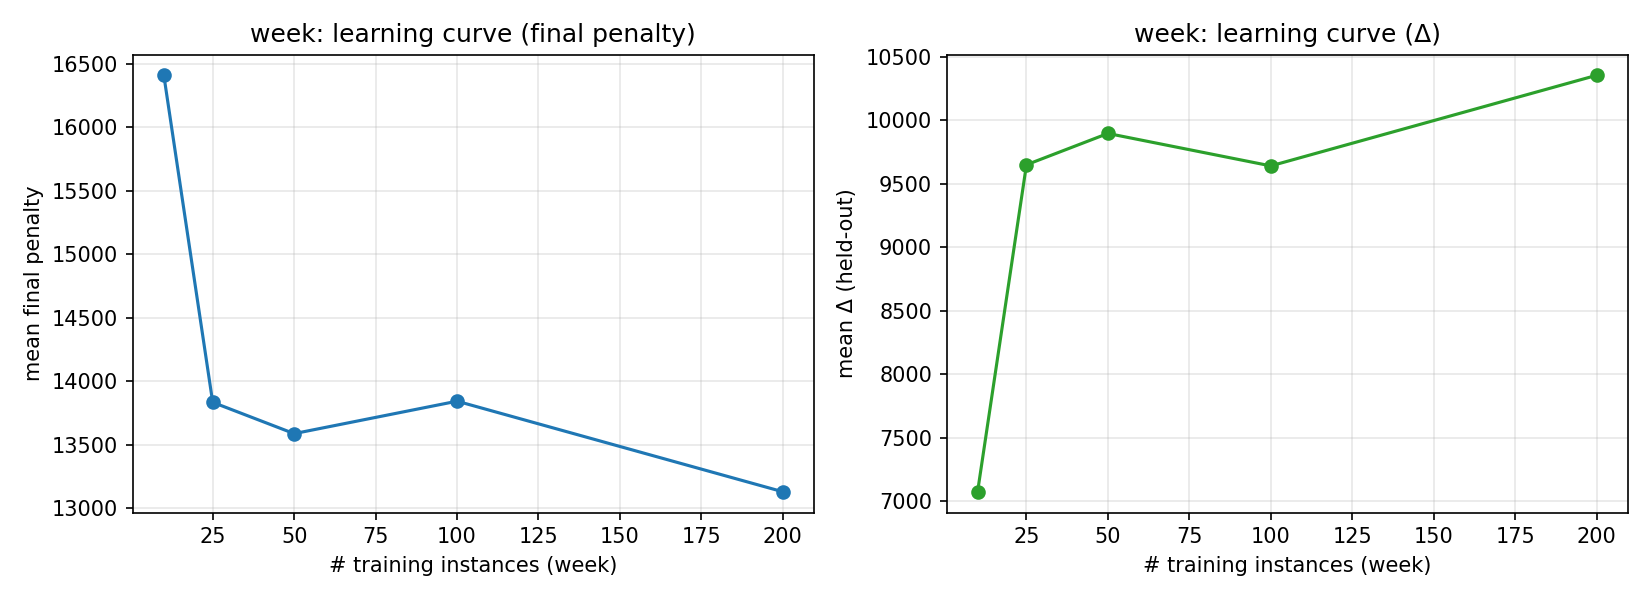
\includegraphics[width=0.48\textwidth]{experiment plots/experiment-06/data_scaling_week.png}
    \hfill
    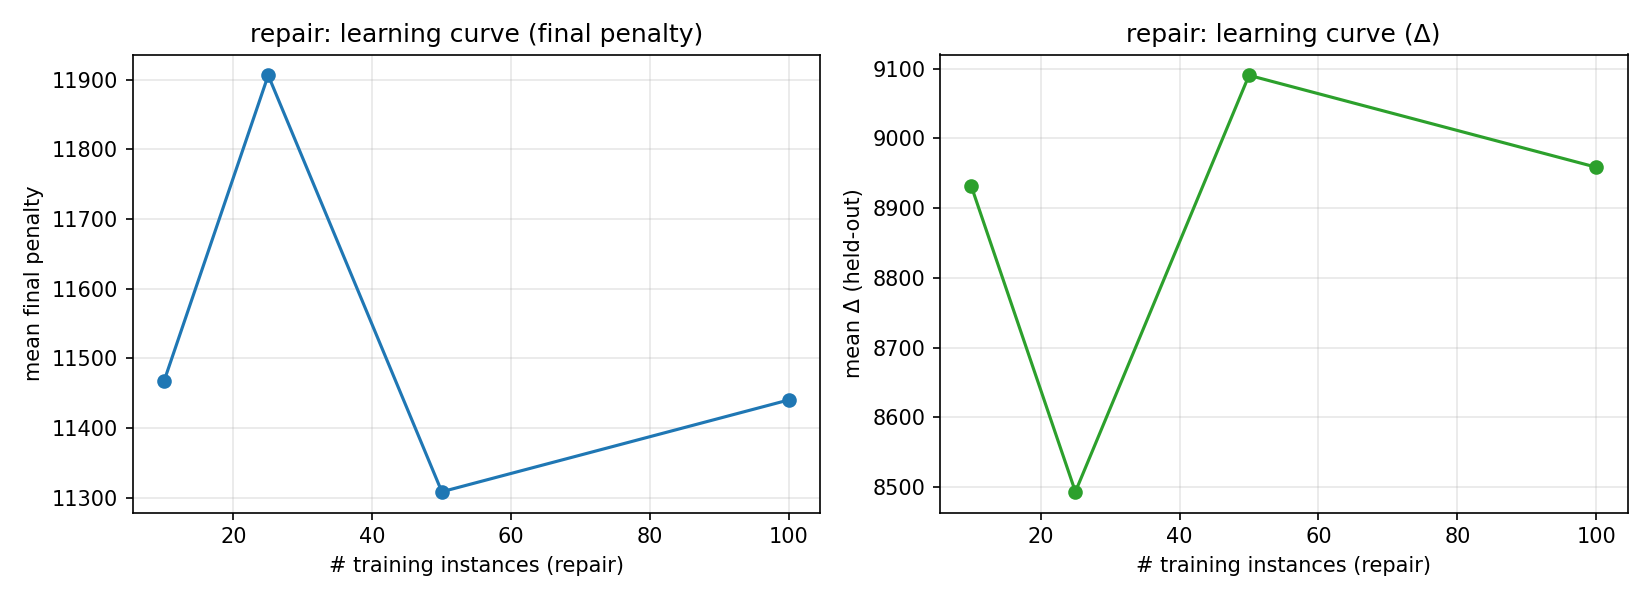
\includegraphics[width=0.48\textwidth]{experiment plots/experiment-06/data_scaling_repair.png}
    \caption{Training-set scaling: held-out dev mean final penalty and mean $\Delta$
    vs.\ number of training instances at the week level (left) and repair level (right).}
    \label{fig:app-data-scaling}
\end{figure}

\end{document}